\documentclass[12pt, t, xcolor=dvipsnames]{beamer}

% draft will print out comment
% final will hide all comment
\usepackage[draft]{pdfcomment}
\usepackage{xspace}
\usepackage{appendixnumberbeamer}
\usepackage{xcolor}
\usepackage{minted}
\usepackage[scale=2]{ccicons}
\usepackage{booktabs}
\usepackage{graphicx}
% \usepackage[absolute,overlay]{textpos}
\usepackage{pgfplots}
\usepackage{amsthm}
\usepackage{amsmath}
\usepackage{tabularx}
\usepackage{centernot}
% \usepackage{hyperref}
% \includeonlyframes{current}

\newcommand{\pdfnote}[1]{\marginnote{\pdfcomment[icon=note]{#1}}}


\useoutertheme{metropolis}
\useinnertheme{metropolis}
\usefonttheme{metropolis}
\usecolortheme{metropolis}

\pgfplotsset{compat=1.14}


\makeatletter
\newcommand*{\indep}{%
  \mathbin{%
    \mathpalette{\@indep}{}%
  }%
}
\newcommand*{\nindep}{%
  \mathbin{%                   % The final symbol is a binary math operator
    \mathpalette{\@indep}{\not}% \mathpalette helps for the adaptation
                               % of the symbol to the different math styles.
  }%
}
\newcommand*{\@indep}[2]{%
  % #1: math style
  % #2: empty or \not
  \sbox0{$#1\perp\m@th$}%        box 0 contains \perp symbol
  \sbox2{$#1=$}%                 box 2 for the height of =
  \sbox4{$#1\vcenter{}$}%        box 4 for the height of the math axis
  \rlap{\copy0}%                 first \perp
  \dimen@=\dimexpr\ht2-\ht4-.2pt\relax
      % The equals symbol is centered around the math axis.
      % The following equations are used to calculate the
      % right shift of the second \perp:
      % [1] ht(equals) - ht(math_axis) = line_width + 0.5 gap
      % [2] right_shift(second_perp) = line_width + gap
      % The line width is approximated by the default line width of 0.4pt
  \kern\dimen@
  {#2}%
      % {\not} in case of \nindep;
      % the braces convert the relational symbol \not to an ordinary
      % math object without additional horizontal spacing.
  \kern\dimen@
  \copy0 %                       second \perp
} 
\makeatother



\newtheorem{mydef}{Definition}

\setbeamercolor{normal text}{fg=black!95, bg=white}
%\setbeamersize{text margin left=6mm, text margin right=6mm} 
\setlength{\leftmargini}{0pt}

\usemintedstyle{borland}

\graphicspath{ {figures/} }

\setbeamercolor{framesource}{fg=gray}
\setbeamerfont{framesource}{size=\tiny}

\makeatletter
\renewcommand{\footnoterule}{}
\define@key{beamerfootnote}{nonumber}[true]{\edef\beamer@footarg{0}\def\@makefnmark{}}% have to set a number in \beamer@footarg, then it won't be automatically generated one. setting \@makefnmark to be empty means the number isn't printed. but only use this in a group else it affects following footnotes!
% instead of 'nonumber', could just use 0 as an optional argument to \footnote, but OP reports that keyval complains about this in some situations
% http://tex.stackexchange.com/questions/89539
\newcommand{\source}[1]{{\footnote[nonumber]{%
    \begin{beamercolorbox}[right,wd=\dimexpr\hsize-1.8em\relax]{framesource}
      \usebeamerfont{framesource}\usebeamercolor[fg]{framesource} Source: {#1}
    \end{beamercolorbox}}}}
\setlength{\footnotesep}{0cm}%\footnotesep is the space between footnotes (generated with a \rule)
\makeatother

% inspired by [beamer: footnote text collides with navigation symbols](http://tex.stackexchange.com/a/5855)
\addtobeamertemplate{sidebar right}{\setbeamertemplate{navigation symbols}{}}{}
\addtobeamertemplate{footline}{\hfill\usebeamertemplate***{navigation symbols}%
    \hspace*{0.1cm}\par\vskip 2pt}{}

% \setbeamercolor{framesource}{fg=gray}
% \setbeamerfont{framesource}{size=\tiny}
% 
% \newcommand{\source}[1]{\begin{textblock*}{4cm}(8.7cm,8.6cm)
%     \begin{beamercolorbox}[ht=0cm,right]{framesource}
%         \usebeamerfont{framesource}\usebeamercolor[fg]{framesource} Source: {#1}
%     \end{beamercolorbox}
% \end{textblock*}}

\tikzset{
  every overlay node/.style={
    draw=black,fill=white,rounded corners,anchor=north west,
  },
}

\def\tikzoverlay{%
   \tikz[baseline,overlay]\node[every overlay node]
}%

\definecolor{codegray}{gray}{0.95}
\newcommand{\code}[1]{\colorbox{codegray}{\textcolor{black!95}{\texttt{#1}}}}
%\newcommand{\code}[1]{\texttt{#1}}}

\newminted{R}{fontsize=\scriptsize, 
              frame=lines,
              bgcolor=codegray,
              framesep=1mm}

\newcommand {\framedgraphic}[2] {
    \begin{frame}{#1}
        \begin{center}
            \includegraphics[width=\textwidth,height=0.8\textheight,keepaspectratio]{#2}
        \end{center}
    \end{frame}
}

\pgfmathdeclarefunction{gauss}{3}{%
  \pgfmathparse{1/(#3*sqrt(2*pi))*exp(-((#1-#2)^2)/(2*#3^2))}%
}

\title{Week 5 Lab}
% \subtitle{}
\date{Tuesday, February 13/Thursday, February 15}
%\author{Yuanchao Zhang}
% \institute{}
% \titlegraphic{\hfill\includegraphics[height=1.5cm]{logo.pdf}}
\renewcommand\appendixname{Appendix}

\begin{document}

\maketitle

\begin{frame}{Plan for today}
\setbeamertemplate{section in toc}[sections numbered]
\begin{minipage}[t][3cm][t]{\textwidth}
  \tableofcontents
\end{minipage}

\end{frame}

\section*{Recap}

\begin{frame}{Recap}
  \begin{itemize}
    \item Risk ratio
    \item Odds ratio
    \item Covariances
    \item Correlation
  \end{itemize}
\end{frame}

\section{Two-sample proportion tests} % (fold)
\label{sec:two_sample_proportion_tests}

\begin{frame}{Overview of two-sample proportion tests}

\begin{itemize}
  \item Scenario: Paired binary data, e.g. the disease and smoke conditions of a study participant. 
  \item Mathematical notation:
  \begin{itemize}
    \item  $(X_1, \ldots, X_n)$ is a sequence of iid random variables of $Bern(p_X)$. Denote as $X^n$.
    \item  $(Y_1, \ldots, Y_n)$ is a sequence of iid random variables of $Bern(p_Y)$. Denote as $Y^n$.
    \item  $((X_1, Y_1), \ldots, (X_n, Y_n))$ is a sequence of paired $X^n$ and $Y^n$. Denote as $(X, Y)^n$.
  \end{itemize}
  \item Data representation: 2 x 2 contingency table
\end{itemize}
\end{frame}

\begin{frame}{2 x 2 contingency table}
\setlength\tabcolsep{3pt}  % default value: 6pt
\small  %%  command to change the font size

\begin{center}

\begin{tabularx}{\textwidth}{@{} X|cc|c @{}}
\toprule
        & $Y=1$ & $Y=0$          & Marginal Total of X \\
\midrule
$X=1$   & $o_{1,1}$ & $o_{1,2}$  &  $o_{1,1} + o_{1,2} = n_{1,*}$ \\ 
$X=0$   & $o_{2,1}$ & $o_{2,2}$  &  $o_{2,1} + o_{2,2} = n_{2,*}$  \\
\midrule
Marginal \newline Total of Y &  $o_{1,1} + o_{2,1} = n_{*,1}$  &  $o_{1,2} + o_{2,2} = n_{*,2}$ \\
\bottomrule
\end{tabularx}
\end{center}

The four entries $o_{1,1}$, $o_{1,2}$, $o_{2,1}$, and $o_{2,2}$  are the observed counts of $(X, Y)^n$. The sum of them is the sample size $n$. 

The column and row sums are called marginal totals. 

\pdfnote{This is like coin flip in 2-sample proportion tests.}

\end{frame}

\begin{frame}{Null hypotheses}
\begin{itemize}
  \item There are mainly three ways to put the same $H_0$:
  \begin{itemize}
    \item $X$ and $Y$ are independent. $H_0$: $X \indep Y$.
    \item The odds ratio is equal to 1. $H_0$: $(o_{1,1} / o_{1,2}) / (o_{2,1} / o_{2,2}) = 1$. 
    \item The proportions of two samples are equal. $H_0$: $o_{1,1} / n_{1,*} = o_{2,1} / n_{2,*}$.
  \end{itemize}
  \item $H_0$: $X \indep Y$ is directly used to derive the test statistic and calculate p-value, but it is equalvalent to the other two $H_0$s.
\end{itemize}
\end{frame}
% section two_sample_proportion_tests (end)



\section{Pearson's chi-square test} % (fold)
\label{sec:pearson_s_chi_square_test}

% \begin{frame}{Pearson's chi-square test}
% \begin{itemize}
%   \item $H_0$: $X \indep Y$.
%   \item $H_a$: $X \nindep Y$.
%   \item Test statistic: $X^{2} = \sum(o_{i,j} - e_{i, j})^{2} / e_{i, j}$, where $e_{i,j} = n_{i,*} \cdot \frac{n_{*,j}}{n}$
%   \item If $H_0$ is true, $X^2 \sim \chi^2(k)$ when $n$ is large, where 
%   \begin{align*}
%   k = & [(\text{number of possible outcomes of } X) - 1] \\
%       & \cdot [(\text{number of possible outcomes of } Y) - 1]\\
%       & \text{(For example, } k = (2 - 1) (2 - 1) = 1  \text{ for }\\
%       & \text{ 2x2 contingency table)} \\
%   \end{align*}
% \end{itemize}
% \end{frame}



\begin{frame}[fragile]{Pearson's chi-square test}
\begin{minted}[fontsize=\scriptsize,
               frame=lines,
               bgcolor=codegray,
               framesep=1mm]{R}
chisq.test(ds_2x2_tbl, correct = F)
## 
##  Pearson's Chi-squared test
## 
## data:  ds_2x2_tbl
## X-squared = 14.613, df = 1, p-value = 0.000132
\end{minted}

\end{frame}

% section pearson_s_chi_square_test (end)



\section{Fisher's exact test} % (fold)
\label{sec:fisher_s_exact_test}

% \begin{frame}{Fisher's exact test}
% \begin{itemize}
%   \item $H_0$: odds ratio is equal to 1. 
%   \item $H_a$: odds ratio is not equal to 1 (two-tailed). 
%   \item Test statistic: $$ p = \frac{ \binom{o_{1,1} + o_{1,2}}{o_{1,1}} \binom{o_{2,1} + o_{2,2}}{o_{2,1}} }
%                                     { \binom{n}{o_{1,1} + o_{2, 1}} }$$
%   \item If $H_0$ is true, $p$ defines a hypergeometric distribution of a random variable $O_{1,1}$, and the probability of observing $o_{1,1}$ is equal to $p$. Denote the probability mass function of the hypergeometric distribution as $P(X=x)$.
%   \item $$\text{p-value} = \sum_{P(X=x) \le P(X=o_{1,1})} P(X=x)$$ 
% \end{itemize}
% 
% \end{frame}



\begin{frame}[fragile]{Fisher's exact test}
\begin{minted}[fontsize=\scriptsize,
               frame=lines,
               bgcolor=codegray,
               framesep=1mm]{R}
fisher.test(ds_2x2_tbl, alternative='two.sided')
## 
##  Fisher's Exact Test for Count Data
## 
## data:  ds_2x2_tbl
## p-value = 0.0001724
## alternative hypothesis: true odds ratio is not equal to 1
## 95 percent confidence interval:
##  0.2584247 0.6776792
## sample estimates:
## odds ratio 
##   0.420428
\end{minted}
\end{frame}

% section fisher_s_exact_test (end)






\section{McNemar's test} % (fold)
\label{sec:mcnemar_s_test}

% \begin{frame}{McNemar's test}
% \begin{itemize}
%   \item $H_0$: $O_{1,2} / n = O_{2,1} / n$. Here, the upper case $O$ indicates that it is a random variable rather than a single observation. 
%   \item $H_0$ is derived from `marginal homogeneity', that is $(O_{1,1} + O_{1,2}) / n = (O_{1,1} + O_{2,1}) / n$. 
%   \item $H_a$: $O_{1,2} / n \neq O_{2,1} / n$. 
%   \item Test statistic: 
% \end{itemize}
% 
% \end{frame}
% 


\begin{frame}[fragile]{McNemar's test}
\begin{minted}[fontsize=\scriptsize,
               frame=lines,
               bgcolor=codegray,
               framesep=1mm]{R}
data <- matrix(c(6, 2, 8, 4), ncol=2, byrow=T)
mcnemar.test(data)
## 
##  McNemar's Chi-squared test with continuity correction
## 
## data:  data
## McNemar's chi-squared = 2.5, df = 1, p-value = 0.1138
\end{minted}
\end{frame}

% section mcnemar_s_test (end)









\section{Kolmogorov-Smirnov Test} % (fold)
\label{sec:kolmogorov_smirnov_test}

\begin{frame}[fragile]{Kolmogorov-Smirnov Test}

\begin{minted}[fontsize=\scriptsize,
               frame=lines,
               bgcolor=codegray,
               framesep=1mm]{R}
x <- rnorm(50) 
y <- runif(30)

ks.test(x,y)
## 
##  Two-sample Kolmogorov-Smirnov test
## 
## data:  x and y
## D = 0.56, p-value = 6.303e-06
## alternative hypothesis: two-sided
\end{minted}
\end{frame}

% section kolmogorov_smirnov_test (end)




\section{qqplots} % (fold)
\label{sec:qqplots}

\begin{frame}[fragile]{qqplots}
\begin{minted}[fontsize=\scriptsize,
               frame=lines,
               bgcolor=codegray,
               framesep=1mm]{R}
x <- rnorm(500)
qqnorm(x)
qqline(x)
\end{minted}

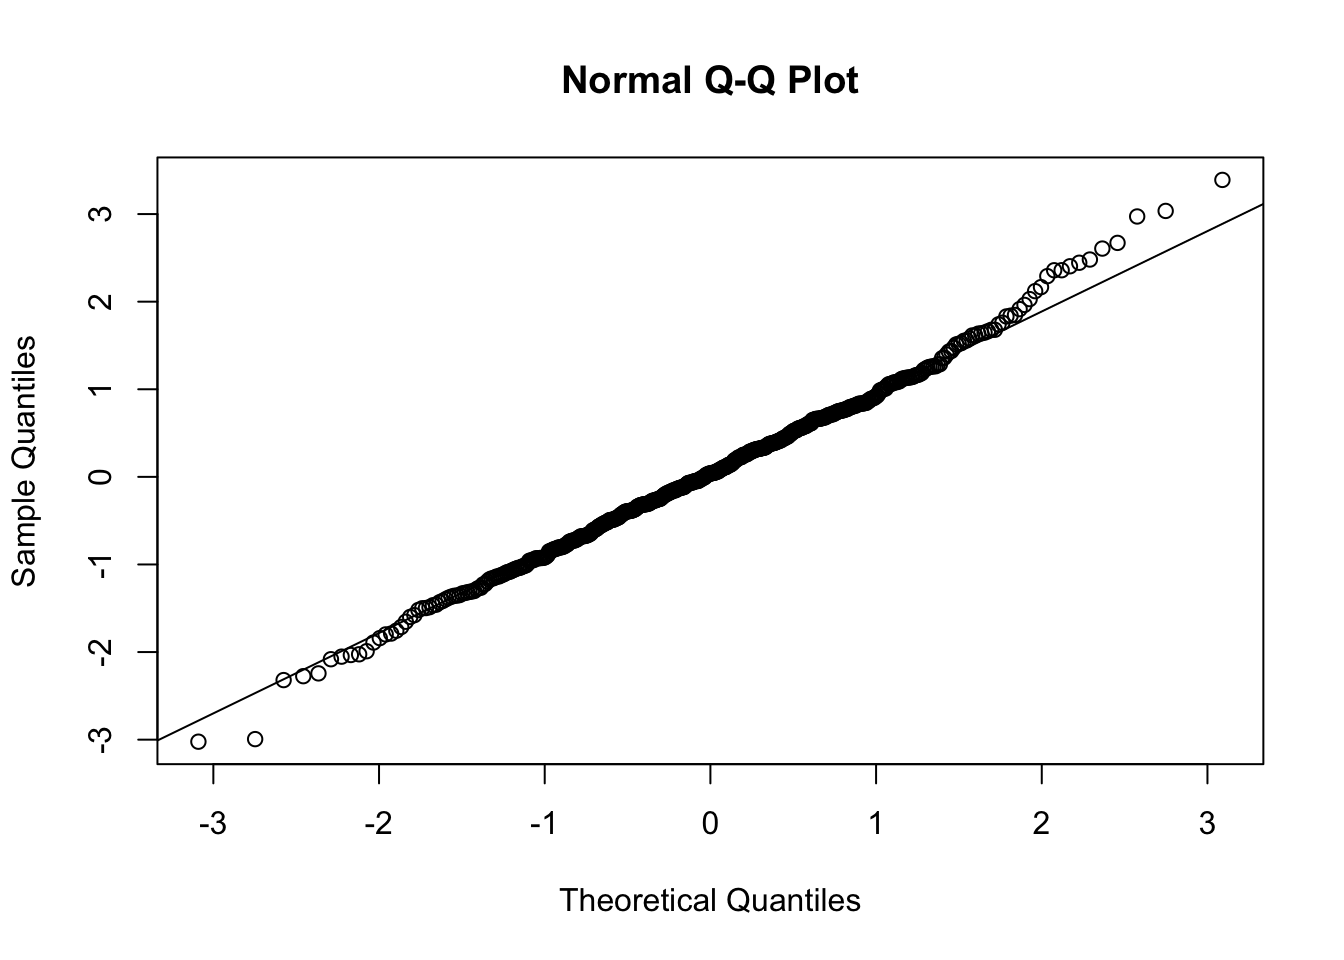
\includegraphics[height=0.5\textheight, keepaspectratio]{rnorm_qqnorm}
\end{frame}

\begin{frame}[fragile]{qqplots}
\begin{minted}[fontsize=\scriptsize,
               frame=lines,
               bgcolor=codegray,
               framesep=1mm]{R}
y <- runif(300)
qqnorm(y)
qqline(y)
\end{minted}

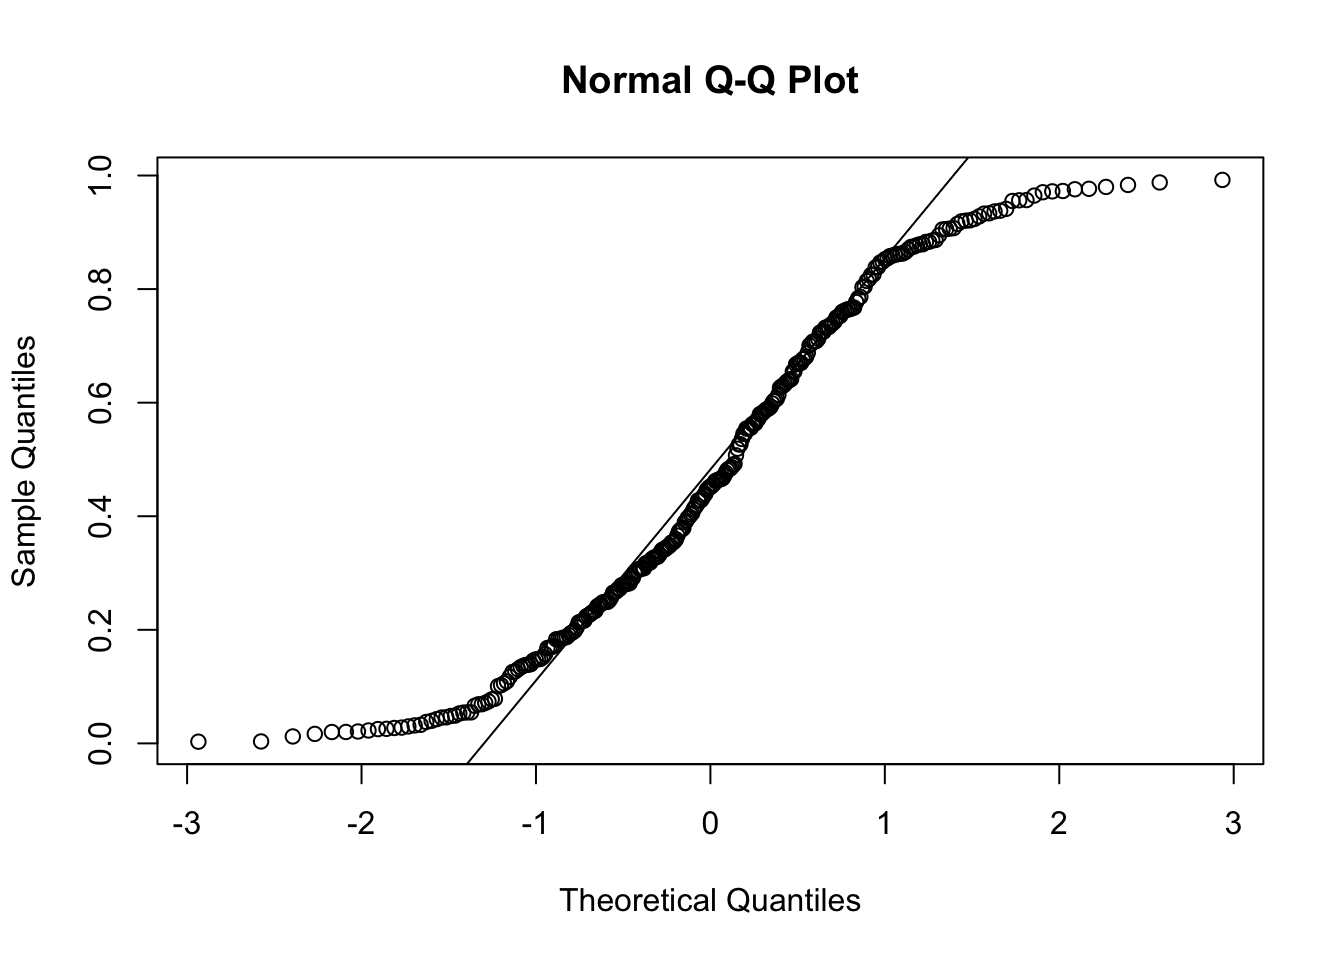
\includegraphics[height=0.5\textheight, keepaspectratio]{runif_qqnorm}
\end{frame}


% section qqplots (end)





\begin{frame}[c]
  \large{Questions?}
\end{frame}


\end{document}
